\begin{figure}[!ht]
	\centering
	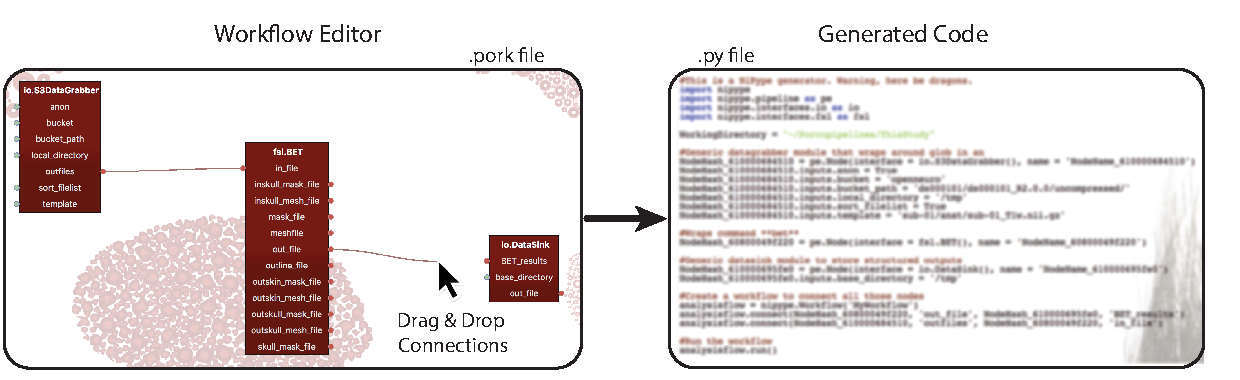
\includegraphics[width=0.9\textwidth, clip=true]{./Chapters/05_Porcupine/./Images/pork_py.pdf}
	\caption{An example of simple workflow. In three steps, this pipeline loads data, processes it, and writes it to disk. This is achieved by connecting the input and output fields from subsequent nodes in the pipeline. The constructed workflow is then transformed in readily executable (Nipype) analysis code.}
	\label{fig:porcupine-simple}
\end{figure}
